\section{System Architecture Design}
\label{Sec-Architecture}

\subsection{System Overview}
Figure \ref{Fig-ContainerVirtualTime} depicts the architecture of our virtual time system within a Linux-container-based network emulator. 
Linux container \cite{LXC} is a lightweight virtualization technique that enables multiple instances of Linux OS sharing the kernel. 
Linux container has less overhead than full or para-virtualization platforms, such as Xen, QEMU, or VMware, in which separated kernels are required for each VM, and therefore, has been applied in the area of scalable network emulation. For example, Mininet \cite{Mininet} is a Linux-container-based emulation platform supporting SDN research. 

Mininet creates containers to virtualize network hosts, and each container has its own private network namespace and interface. Applications (such as web services) are encapsulated in the containers. The containers are connected by software switches (typically kernel-model Open vSwitch \cite{OpenvSwitch}) with virtual interfaces and links as shown in Figure \ref{Fig-ContainerVirtualTime}, and are multiplexed onto the physical machine. Like many other network emulators, Mininet is also vulnerable to the temporal fidelity issue in large-scale network experiments. Containers use the same system clock of the physical machine, but the execution of the containers is scheduled by the OS in serial. This leads to incorrect perception of time in a container, because the container's clock keeps advancing even if it is not running (e.g., idle, waiting, suspended). Such errors are particularly severe when emulating high workload network experiments.

To improve the temporal fidelity, we build a virtual time system as a lightweight middleware in the Linux kernel (see Figure \ref{Fig-ContainerVirtualTime}). We employ the time dilation technique to provide the illusion that a container has as much processing power, disk I/O, and network bandwidth as a real physical host in a production network despite the fact that it shares the underlying resources with other containers. The basic idea is to make time appear to be slower than the wall-clock time, so that the emulated network appears faster.

A capable virtual time system for scalable network emulation needs to have the following requirements: (1) lightweight design with low system overhead, (2) transparent virtual time provision to applications in containers, i.e., no code required modification,  (3) universal virtual time support within the emulator and invisible to other processes on the same machine, and (4) ease of integration to the emulator. Accurate and positive emulation results can improve the confidence that any changes (e.g., a transformation from a traditional network to an SDN-based architecture) to the target production network will be successfully deployed. 

\begin{figure*}
\centering
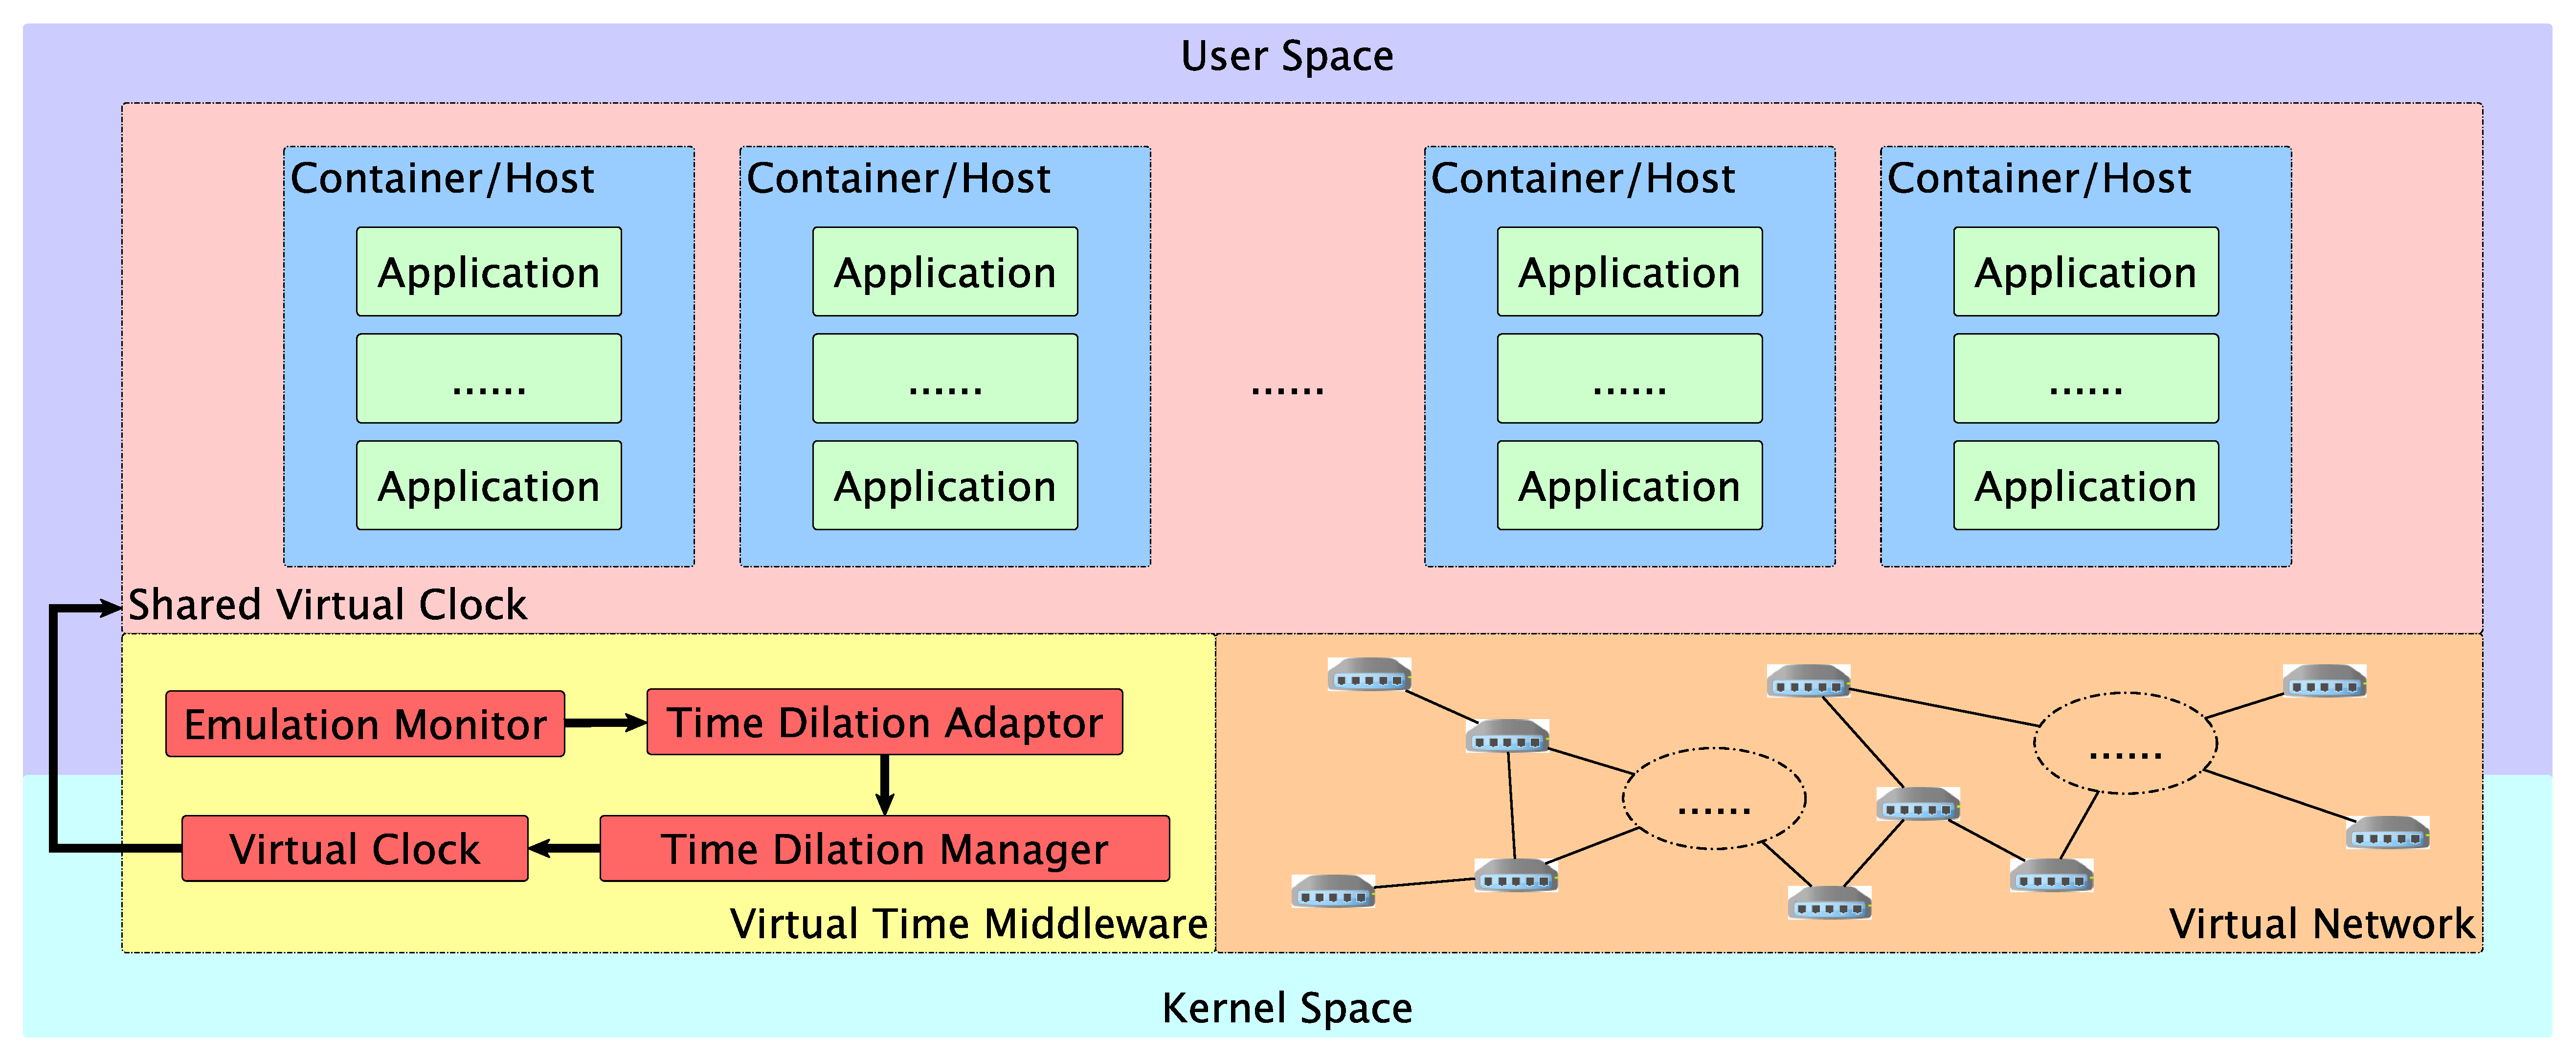
\epsfig{file=figures/ContainerVirtualTime.eps, height=2in, width=5in}
\caption{\textbf{Architecture of the Virtual Time System in a Container-based Network Emulator. Note that a typical container-based network emulator can be presented by this figure without the Virtual Time Middleware.}}
\label{Fig-ContainerVirtualTime}
\end{figure*}

\subsection{Virtual Time Management}
Our virtual time system, as shown in Figure \ref{Fig-ContainerVirtualTime}, is designed to meet all the requirements. The time dilation manager is responsible for computing and maintaining the virtual time, according to a given TDF for all the containers. It can offer per-container virtual time or the global virtual time for the emulator. The per-container virtual time is useful to support synchronized emulation (in virtual time) and facilitates the integration with network simulators. We have made a small set of changes in the kernel, in particular, a modified data structure to present virtual time, and a new algorithm to convert the elapsed wall-clock time to the dilated virtual time, with no dependency on third-party libraries.

We attach each container an integer-valued TDF, which could also be shared among all containers. A TDF of $k$ slows down a container's time advancement rate by a factor of $k$, thus re-scales a container's notion of time with reference to a physical network. This way, Mininet can emulate a seemingly $k$ times faster network owing to the accelerated rate of interaction between the containers and the virtual network
%When TDF is greater than 1, it appears to the containers that available resources including link bandwidth and CPU computation capacity are increased by a factor of TDF. 
Note that our design cannot scale the capacity of hardware components such as main memory, processor caches, and disk, firmware on network interfaces. 

The integration with Mininet, and potentially other container-based software is straightforward. We provide a set of simple APIs to (1) initialize containers with virtual time, and (2) inquire virtual time at run time. The system returns precise virtual time to container processes and transparently to all their child processes while returning the ordinary system time to other processes. We have integrated the system with Mininet. The implementation details are discussed in Section \ref{Sec-Implementation}, and we plan to make our code base available to public on GitHub soon. 

\subsection{Adaptive Time Dilation}

The key insight of virtual time is to trade time with available system resources. The execution time can be unnecessarily long with an overestimated TDF. It is difficult to avoid that with a fixed TDF when the resource demands vary substantially during the emulation. Therefore, we investigate means to adaptively adjust TDF in run-time with the goal of well balancing the execution speed and accuracy. We take a similar epoch-based approach described in \cite{NtwkEmultAdaptVirtTime}, and develop two modules, Emulation Monitor and Time Dilation Adaptor (see Figure \ref{Fig-ContainerVirtualTime}), to achieve the dynamic TDF adjustment. 

Emulation Monitor periodically collects the process-related information (not necessarily coincides with the epoch duration) and computes the run-time emulation load statistics, such as CPU utilization, number of waiting processes, or average process waiting time. Time Dilation Adaptor takes the inputs from Emulation Monitor, and adaptively computes the TDF for the next epoch based on a heuristic algorithm, whose details are presented in Section \ref{Sec-Implementation}. Currently we only use the CPU utilization as the feedback control indicator, and will leave the exploration of other control algorithms as future works. 

% Figure \ref{Fig-ContainerVirtualTime} presents the simplified structure of a regular container-based emulator if we eliminate all the parts inside the yellow rectangle. Usually, emulator will create container for each virtual host and later put the application that runs on a particular host into the correct container. As the key different from other virtualization techniques, container-based host share the guest OS's kernel; they are no different than a special process that think itself as the owner of the machine. In practice, it will be more efficient to put virtual network, including virtual switches, virtual interfaces and link, inside the kernel space. However, user space virtual network is also an option.

% Figure \ref{Fig-ContainerVirtualTime} also describes what the original architecture becomes after we add virtual time and dynamic time dilation management features in to the emulator. Since the only difference between with and without virtual time support is constrained inside the yellow part only, users can run previous experiments in no need of virtual time without any modification. To fulfill backward-compatibility, we add a middleware between (and inside) kernel and the containers application resides in. Such a design can let users execute applications or experiments that DOES need virtual time. If one wants to run his or her emulation with virtual time enabled, all one needs to do is to either feed a fixed time dilation factor or simply specify an dilation adaptor so that our system can take care of the dilation configuration from then on. In the term of software architecture, the network emulator with virtual time support can been seen as a 3-layered software: the Application Layer that includes containers and applications, the Virtual Time Management Middleware and OS Kernel Layer. We describe each layer one by one.

% \begin{figure*}
% \centering
% 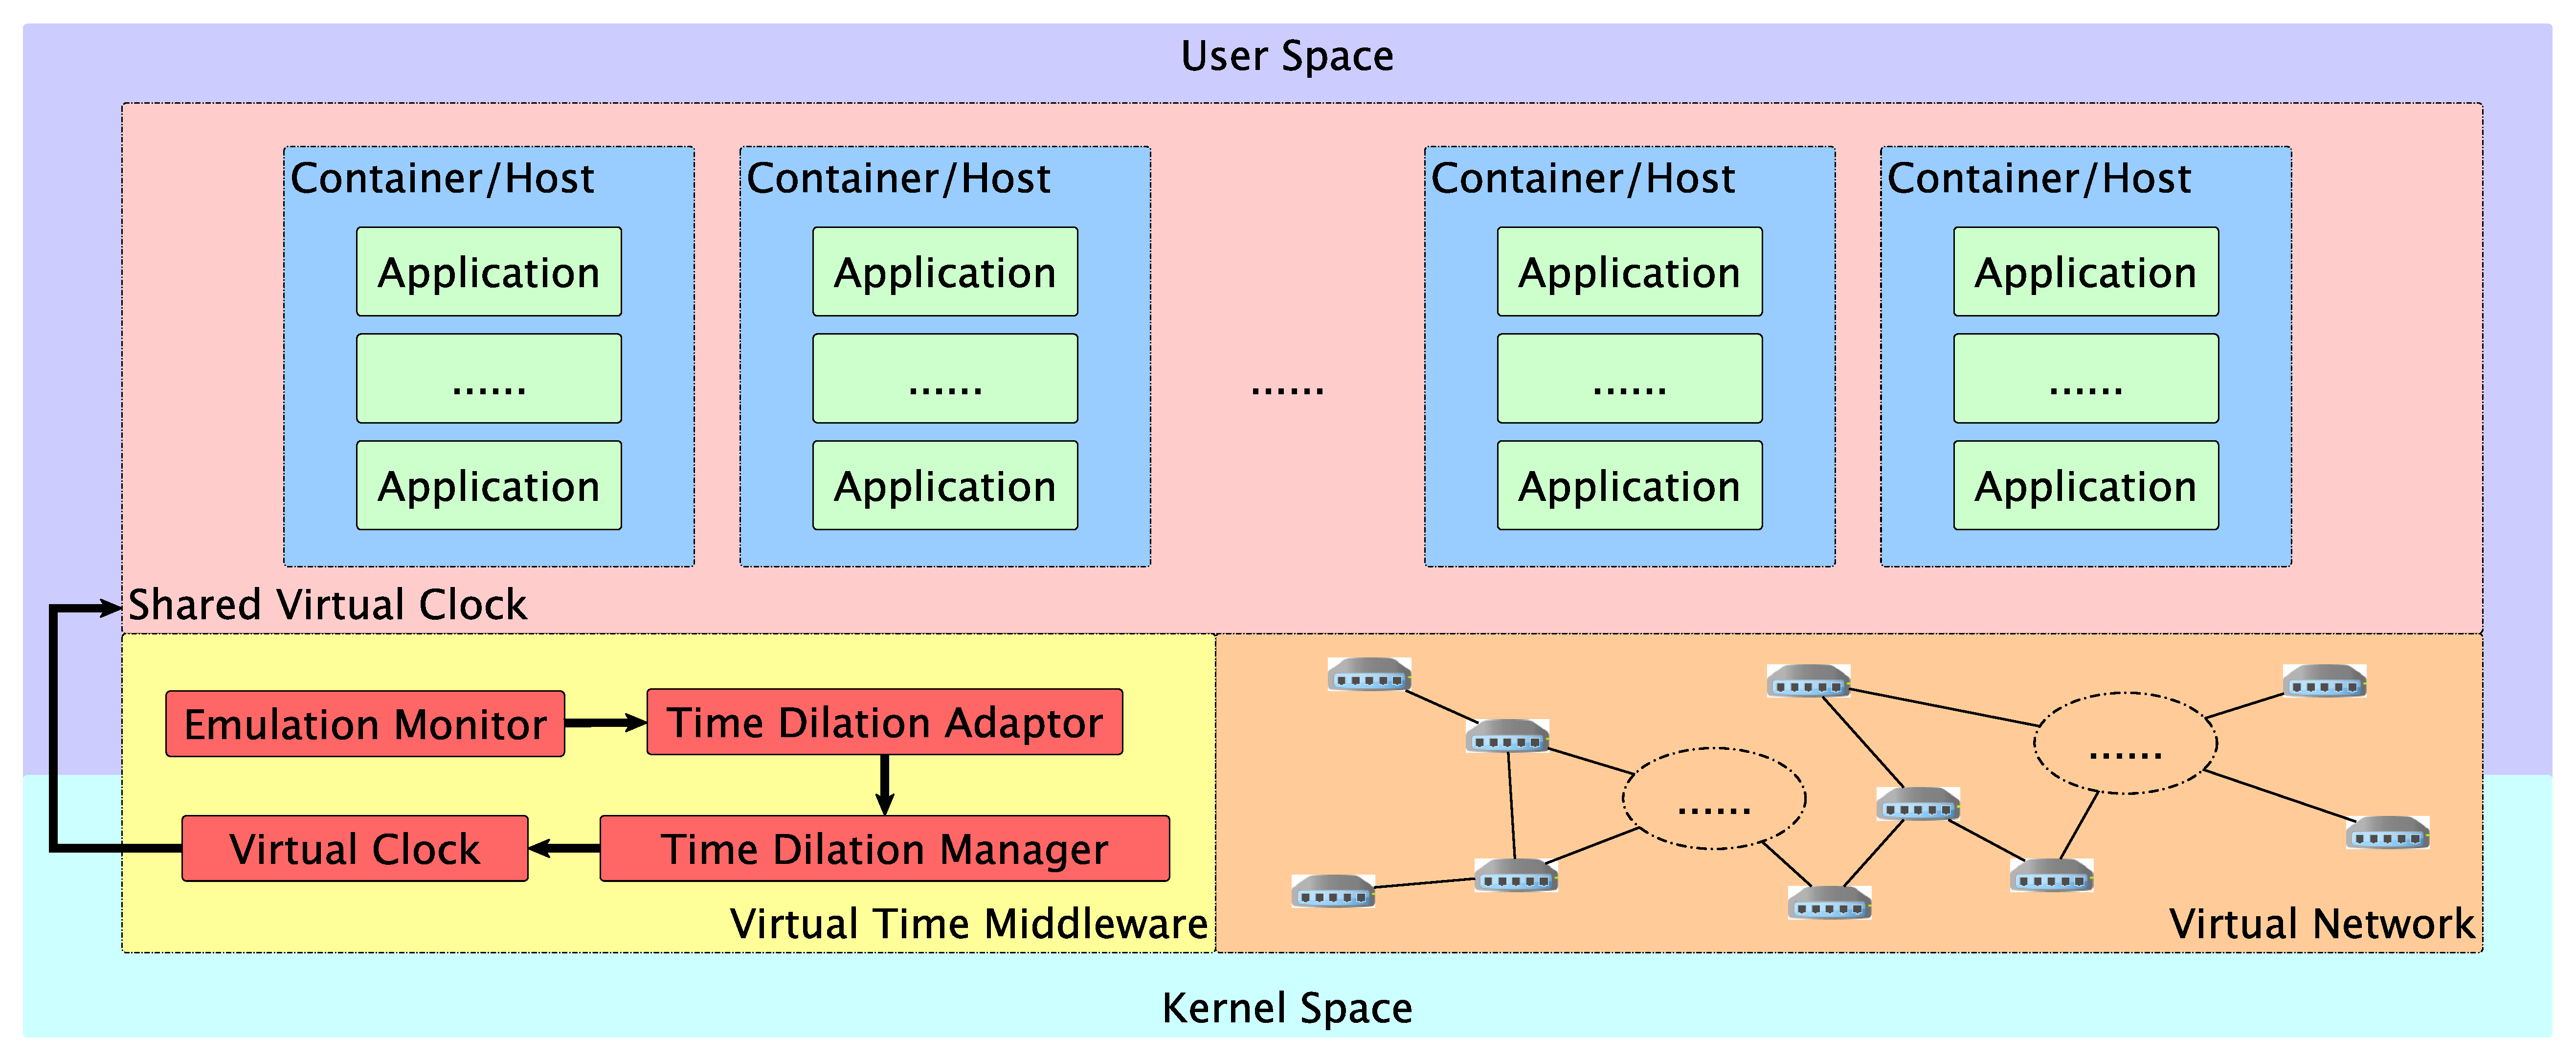
\epsfig{file=figures/ContainerVirtualTime.eps, height=2in, width=5in}
% \caption{\textbf{Virtual Time System Architecture Design with Integration of a Container-based Network Emulator}}
% \label{Fig-ContainerVirtualTime}
% \end{figure*}

% \subsection{OS Kernel Layer}
% In this layer, as shown in Figure \ref{Fig-ContainerVirtualTime}, we need to modify the kernel itself so that it has a virtual clock, e.g. the Virtual Time Supported Kernel. This involve patching many parts in the original kernel. For example, we should add data structures to present the virtual time, add algorithms to calculate virtual time from real time. Besides, in order to further schedule the speed of the Virtual Clock, a Time Dilation Management mechanism is a must. Those new features provided by modified kernel is available through new defined kernel APIs. Typically, we need to add an API to create a process that use virtual clock and an API to change a process's virtual clock speed. Returning virtual time to containers should use the old API that kernel uses when returning wall clock time. Only in this way can all the modifications be transparent to arbitrary applications.

% \subsection{Virtual Time Management Middleware}
% \label{Sub-Sec-VirtualTimeMiddleware}
% This layer exists as a service layer for applications that the users are interested to test with virtual time. If a user is willing to provide a time dilation because he or she already knows that the underlying hardware resource is not sufficient to run a experiment with high fidelity, emulator can accept it and enable virtual time right from the beginning of the emulation. Otherwise, our virtual time supported emulator is able to take care of the speed of the experiment for the users. That is to say, emulator have the freedom to choose a time dilation as large as possible such that experiment environment is scaled to the physical one that the user wants. However, it also have the responsibility to finish the experiment as soon as possible or report impossible to finish the experiment because it will take too long.

% In order to provide these features to user, our system borrows the concept of \textit{Epoch} from \cite{NtwkEmultAdaptVirtTime} to schedule time dilation factor. During an epoch, all virtual nodes in emulation run under the same constant TDF. Upon entering an new epoch, the emulator has the chance to tune the global TDF for itself. Epochs, naturally, should have distinguished characters of load, which measured by the system utilization, usually percentage of CPU time in practice.

% To collect load statistics of an Epoch and deal with the Epoch transition, we should have 2 modules in the virtual time management subsystem: Emulation Monitor and Time Dilation Adaptor. The Emulation Monitor polls OS periodically (may not coincides with Epoch's duration) and get comprehensive statistics that reflect the system load at run-time. In a container based network emulator, usually virtual nodes (including hosts, switches and controllers in a typical SDN network environment) are all processes inside independent containers; every application is being executed as child process of the node it runs on. Since containers are naturally separated from other processes in the same OS, it is quiet convenient to gather the load statistics only related to emulator. Using these information, emulator could consult Time Dilation Adaptor who returns an appropriate time dilation grounded on some heuristic algorithm. It can be as intuitive as the one in \cite{NtwkEmultAdaptVirtTime}. Note that changing TDF for a container actually happens in kernel space; emulator simply delegate this task to OS Kernel Layer who does the dirty works. 

% Our dynamic time dilation management system actually shares many concepts proposed by \cite{NtwkEmultAdaptVirtTime}, though the relation between Monitor and Adaptor in our design is different from theirs. However, the differences in implementation are significant. We will discuss these differences in subsection \ref{Sub-Sec-ImplementMininet}.

% \subsection{Application Layer}
% Emulator can directly create containers that virtualize network hosts. Each container has its own private network namespace/interface. After introducing virtual routing or virtual switch technique, a non-trivial network environment can be build upon a single machine. All containers are sharing the same virtual clock that can be faster or slower than the clock OS kernel uses. As for now, it only makes sense that all containers use virtual clocks of the same advance speed, e.g. share global time dilation factor. When using a time dilation factor (TDF) greater than 1, it appears to host that available resources, for example, link bandwidth and CPU computation capacity, increase to TDF times. However, as one of the most obvious and serious problem of virtual time, all the emulated hosts running TDF times slower now. Sometimes we can do nothing about it but notify user that the emulation have to take that long time because a smaller dilation cannot guarantee the target experiment environment. Fortunately, our Virtual Time Management Middleware can mitigate this problem in the cases that user feed an overestimated time dilation factor, or the resource demand varies during the emulation.

% Directly or indirectly, applications are developed on the basis of the APIs operating system exposed to the outside world. They are often kicked off by emulator. When adopting the design in Figure \ref{Fig-ContainerVirtualTime}, we do not need to modify anything in the applications; applications still ask for anything they need through the same API from software library or OS kernel, for example, asking for time. 
